
%(BEGIN_QUESTION)
% Copyright 2010, Tony R. Kuphaldt, released under the Creative Commons Attribution License (v 1.0)
% This means you may do almost anything with this work of mine, so long as you give me proper credit

Sketch connecting wires such that the relay will de-energize and turn on the lamp when the normally-closed (NC) pushbutton switch is pressed.  Use the following schematic diagram as a guide:

$$\includegraphics[width=15.5cm]{i02233x01.eps}$$

Note how the relay coil and lamp are separate (parallel) branches in this circuit.  The pushbutton switch {\it only} carries coil current, while the relay's switch contact {\it only} carries lamp current.

\vfil 

\underbar{file i02233}
\eject
%(END_QUESTION)





%(BEGIN_ANSWER)

This is a graded question -- no answers or hints given!

%(END_ANSWER)





%(BEGIN_NOTES)

Note how a schematic diagram was provided for you, to help you determine where each and every wire should go.  In real-life situations, you may not be given any schematic diagram at all.  In such cases, it is an excellent problem-solving strategy to first sketch your own schematic diagram, before attempting to sketch a pictorial diagram or connect real wires to the devices.  The concept here is that schematic diagrams are much easier to interpret and understand than pictorial diagrams where wires tend to cross over each other more, and where components are not always optimally placed.

\vskip 10pt

Bear in mind that this is not the {\it only} possible circuit solution:

$$\includegraphics[width=15.5cm]{i02233x02.eps}$$

Note that we are using the normally-closed (NC) contact on the relay, in order for the logical ``truth'' of the circuit to be correct.  Since the pushbutton switch itself is normally-closed, and we wish the lamp to energize when we push the switch, the relay needs to be logically inverted as well.

%INDEX% Pictorial circuit review (relay circuit)

%(END_NOTES)


